
Most of the data about the skew quadrupole is presented in Section~\ref{section: 1d_quench_propagation_geometry}. Figure~\ref{fig:skew_quad_transversal_cross_section} shows the transversal cross-section of one coil of the skew quadrupole. The coil is enclosed within an area of 24.5x27.3~mm covered with a 1 mm-thick ground insulation layer. The ground insulation is made of BT-S2, being a mixture of resin and S2-glass provided by the Arisava company~\cite{arisawa_company}. The~thickness of the~ground insulation on the~internal side of a~coil is lower and equal to 0.15~mm.

\begin{figure}[H]
    \centering
    \begin{tikzpicture}[scale=0.8]
    \pgftext{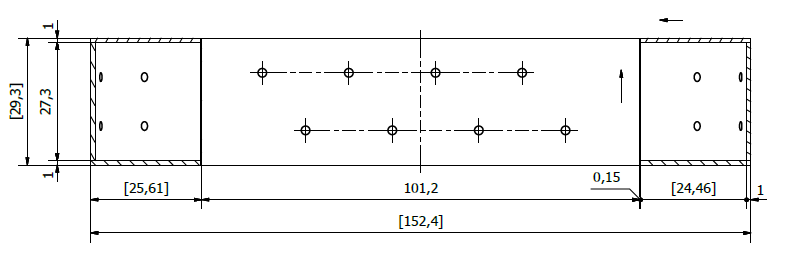
\includegraphics[width=\linewidth]{sections/skew_quad_q_det/figures/skew_quad_design/skew_quad_transversal_cross_section.png}} at (0,0);
    \node[red, scale=0.8] at (6.05,2.1) {layers};
    \node[red, rotate=90, scale=0.8] at (4.3,0) {turns};
    \draw[red, very thick, dashed] (0.47,-0.95) -- (0.47,2.4); 
    \node[red, scale=0.8] at (1.9,2.1) {coil symmetry};
    \draw[black, very thick, ->] (-4.3,2.1) -- (-4.8,1.8); 
    \node[black, scale=0.8] at (-2.65,2.1) {ground insulation};
    \end{tikzpicture}
    \caption{The transversal cross-section of one coil of a skew quadrupole~\cite{samuele_mariotto_mails}.}
    \label{fig:skew_quad_transversal_cross_section}
\end{figure}

The remaining dimensions of the coil are shown in its top view in Fig.~\ref{fig:skew_quad_top_view}.

\begin{figure}[H]
    \centering
    \begin{tikzpicture}[scale=0.8]
        \pgftext{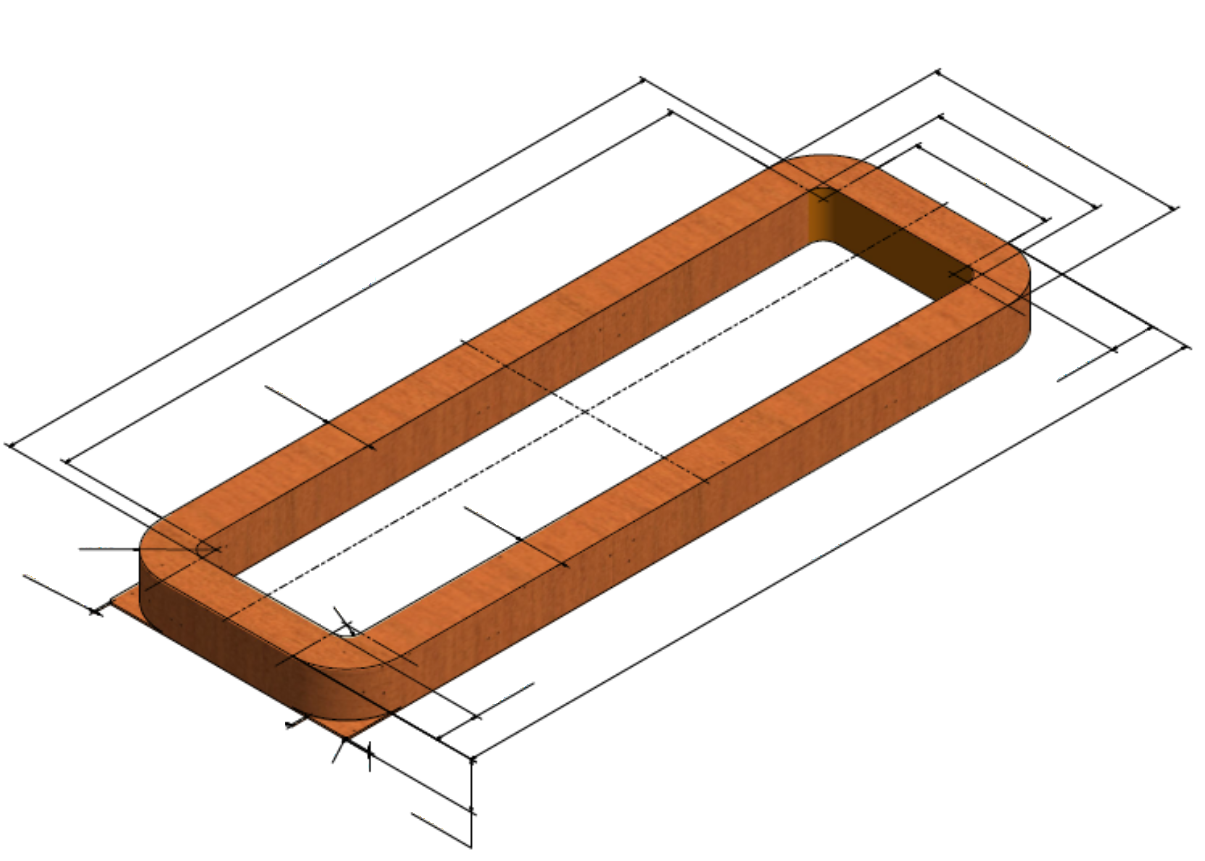
\includegraphics[width=\linewidth]{sections/skew_quad_q_det/figures/skew_quad_design/skew_quad_top_view.png}} at (0,0);
        
        \node[black, rotate=30, scale=0.8] at (-3,2.04) {387.6};
        \node[black, rotate=30, scale=0.8] at (-3.5,2.35) {405.6};
        \node[black, rotate=30, scale=0.8] at (3,-1.23) {$456.8 \pm 0.3$};
        
        \node[black, rotate=-30, scale=0.8] at (4.85,3.33) {83.2};
        \node[black, rotate=-30, scale=0.8] at (5.3,3.6) {101.2};
        \node[black, rotate=-30, scale=0.8] at (5.8,3.85) {$152.4 \pm 0.15$};
        
        \node[black, scale=0.8] at (-6.5,-1.28) {R34.81};
        \node[black, rotate=30, scale=0.8] at (-3.35,-1.96) {R9};
        \draw[black] (-3.4,-2.25) -- (-3,-2); 
        
    \end{tikzpicture}
    \caption{Top view of a skew quadrupole wrapped with the ground insulation~\cite{samuele_mariotto_mails}.}
    \label{fig:skew_quad_top_view}
\end{figure}

As shown in Fig.~\ref{fig:winding_arrangement_cross_section}, each coil has 29 turns in each of its 26 layers. In total, the number of windings per coil is 754~\cite{hl_lhc_tech_design_report_v01}.

\begin{figure}[H]
\centering
    \begin{tikzpicture}
        \begin{axis}[
          width=0.5\linewidth, 
          height=0.5\linewidth,
          xtick={0.0, 24.46},
          ytick={0.0, 27.30},
          xlabel={$x,~\text{mm}~\text{(layers direction)}$},
          ylabel={$y,~\text{mm}~\text{(turns direction)}$},
          xmajorgrids=true,
          ymajorgrids=true,
          xmin=-5.0,
          xmax=29.47,
          ymin=-5.0,
          ymax=32.29,
          ]
          \addplot[blue, only marks, mark size=1pt] table[x=x,y=y,col sep=comma] {sections/skew_quad_q_det/figures/skew_quad_design/winding_location_cross_section.csv};
        \end{axis}
        \draw[scale=0.172, red, very thick, dashed] (2.5,2) -- (2.5,33.0); 
        \node[red, scale=0.8] at (1.9,5.6) {coil symmetry};
        
    \end{tikzpicture}
    \caption{Location of the windings in the cross-section of a half-coil.}
    \label{fig:winding_arrangement_cross_section}
\end{figure}

The winding scheme is shown in Fig.~\ref{fig:winding_scheme_cross_section}. The winding~1 is placed at the bottom left of the 2D cross-section. The last winding number 754 is placed further in the \textit{x}-direction. The~\nth{2} half of the coil is a~mirror reflection of the presented winding scheme.~\cite{marco_prioli_mails}

\begin{figure}[H]
\centering
    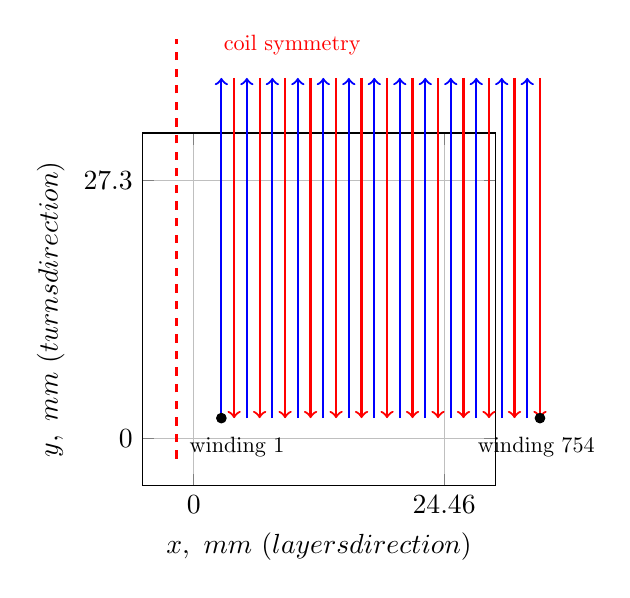
\begin{tikzpicture}
        \begin{axis}[
          width=0.5\linewidth, 
          height=0.5\linewidth,
          xtick={0.0, 24.46},
          ytick={0.0, 27.30},
          xlabel={$x,~\text{mm}~\text{(layers direction)}$},
          ylabel={$y,~\text{mm}~\text{(turns direction)}$},
          xmajorgrids=true,
          ymajorgrids=true,
          xmin=-5.0,
          xmax=29.47,
          ymin=-5.0,
          ymax=32.29,
          ]
        \end{axis}
        \foreach \t in {0.471, 2.353,...,24}
            \draw[scale=0.172, blue, thick, ->] (\t+5.35,5.0) -- (\t+5.35,26.819+3.3); 
        \foreach \t in {1.412, 3.294,...,25}
            \draw[scale=0.172, red, thick, ->] (\t+5.35,26.819+3.3) -- (\t+5.35,5.0);
        \draw[scale=0.172, red, very thick, dashed] (2.5,2) -- (2.5,33.0); 
        \node[red, scale=0.8] at (1.9,5.6) {coil symmetry};
        \filldraw[scale=0.172, black] (0.471+5.35,5.0) circle (10pt);
        \node[black, scale=0.8] at (1.2,0.5) {winding 1};
        \filldraw[scale=0.172, black] (23.996+5.35,5.0) circle (10pt);
        \node[black, scale=0.8] at (5.0,0.5) {winding 754};
        
    \end{tikzpicture}
    \caption{Winding scheme of a single coil of the skew quadrupole.}
    \label{fig:winding_scheme_cross_section}
\end{figure}

Unlike in the analyses with a single strand presented in previous chapters, when a multi-strand thermal simulation of a magnet is considered, it is important to specify its winding scheme because the windings interact with each other thermally across the insulation layer. The general parameters of the skew quadrupole are summarised in Table~\ref{table:skew_quad_params_table}. Four coils of the magnet are connected in series and powered by a single power converter. The coil length, being a quarter of the total strand length of the entire magnet, is more than 812~m. It is a very large number for thermal quench simulations, as mentioned in Section~\ref{section: 1D_quench_propagation_conclusions}. The~operating current of the skew quadrupole is $I=174~\text{A}$.

\begin{table}[H]
    \caption{Geometrical parameters of the skew quadrupole \cite{hl_lhc_tech_design_report_v01, marco_prioli_mails}.}
    \vspace{-1.em} 
    \fontsize{10}{10}
    \selectfont 
    \renewcommand{\arraystretch}{1.5}
    \begin{center}
    \begin{tabular}{ ccc }  
    \hline
    parameter & value & unit \\
    \hline
    number of circuits & 1 & [-] \\
    $L_\text{coil}$ & 812 & [m] \\
    $I_\text{operating}$ & 174 & [A] \\
    \hline 
    \end{tabular}
    \end{center}  
     \label{table:skew_quad_params_table} 
 \end{table}